% vim: tw=80

\chapter{Measurement of the Triple-Differential Dijet Cross Section}

\section{Observable definition}

\section{Datasets}
\label{sec:datasets}

\subsection{Data Samples}

Within the run 1 of the data-taking at the LHC, the CMS experiment collected in
2012 data at a center-of-mass energy of $\sqrt{s} = 8 \si{\TeV}$. The data
sample corresponds to a total integrated luminosity of $\mathcal{L} = 19.71
\si{\fbinv}$. The events are streamed into different primary datasets based on
the trigger decision. All data triggering the prescaled or unprescaled jet
triggers were assigned to the \texttt{JetMon} or \texttt{JetHT} primary
datasets, respectively. The datasets are split into multiple samples
corresponding to the period of data taking in 2012, called Run A,B,C and D.
Unfortunately the trigger assignment to the primary datasets changed during the
data taking period, as can been seen in Table~\ref{tab:datasets}, it was taken
care to avoid any double counting. While in run A all events were stored in the
dataset \texttt{Jet}, the prescaled and unprescaled triggers were split into
separate streams \emph{JetMon} and \emph{JetHT} in the runs B, C and D.

\begin{table}[htbp]
    \centering
    \begin{tabular}{llll}
    \toprule
    Run & Run Range & Dataset & Luminosity (\si{\fbinv})\\\midrule
    A & 190456--193621 & /Jet/Run2012A-22Jan2013-v1/AOD & 0.88\\
    B & 193834--196531 & /Jet[Mon,HT]/Run2012B-22Jan2013-v1/AOD & 4.49\\
    C & 198022--203742 & /Jet[Mon,HT]/Run2012C-22Jan2013-v1/AOD & 7.06 \\
    D & 203777--208686 & /Jet[Mon,HT]/Run2012C-22Jan2013-v1/AOD & 7.37\\ 
    \bottomrule
    \end{tabular}
    \caption{The full 2012 dataset is used. In Run A, events of all single jet trigger paths are stored in 
        the stream Jet, while the prescaled triggers were moved to the JetMon stream in the runs
        B, C and D. Events triggering the unprescaled trigger are in the stream
    JetHT.}
    \label{tab:data:datasets}
\end{table}

\subsection{Monte Carlo Samples}

To compare the data distributions with simulated events, two Monte-Carlo event
generators were considered. An overview about the Monte-Carlo generators is
given in Section~\ref{subsection:mc_generators}. Each MC generator is using and
optimized tune to simulate the underlying event. Additionally the data samples
contain not only the hard interaction but also a model for pile-up collionsion,
through which additional soft scattering events following the pile-up
distribution in data are mixed into the event. 

The Madgraph+P6 sample is a multi-leg improved HT-binned sample. By using
Madgraph, the LO matrix elements not only contain the $2 \rightarrow 2$ matrix
elements, but also the $2 \rightarrow 3$ matrix elements better describing
multijet events. The underlying event is modelled using the tune $Z2*$. The
parton shower and hadronization is carried out using the Pythia 6 event
generator which is interfaced to Madgraph using the LHE event record.

Additionally a Pythia 8 data sample is analyzed. While including only the $2
\rightarrow 2$ LO matrix elements, the event simulation and the underlying event
tune are improved in this newer Pythia version. Both Monte-Carlo samples are
processed through the complete CMS detector simulation to allow studies of the
detector response and compare to the measured data on detector level. 

\begin{table}[htp]
    \centering
    \begin{tabular}{llll}
    \toprule
    Dataset Name & Dataset identifier & Number of events\\\midrule
    MG+P6 & /QCD\_HT-XXToXX\_TuneZ2star\_8TeV-madgraph-pythia/Summer12\_DR53X-PU\_S10\_START53\_V7A-v1/AODSIM & \\
    P8 & QCD\_Pt-XXtoXX\_Tune4C\_8TeV\_pythia8/Summer12\_DR53X-PU\_S10\_START53\_V7A-v1/AODSIM & \\
    \bottomrule
    \end{tabular}
    \caption{Official MC production samples used in the analysis.}
    \label{tab:montecarlo:datasets}
\end{table}

Since the jet spectra steeply fall with increasing \pt it is not possible to
generate a high number of high-\pt events in a reasonable time.  Therefore the
event generation is split into different phase space region binned in HT, the
scalar sum of the jet \pt, or the leading jet \pt. The different phase space
regions are then stitched together later in the data analyses while taking into
account the cross section in the different phase space regions.
Table~\ref{tab:montecarlo:datasets} shows the used data sets and the number of
events per dataset.

\section{Event selection}

\subsection{Certified Data Selection}

The first step in the event processing chain is to only pick runs and
luminosity sections (LS) which fullfill certain criteria. These include the
proper performance of all detector subsystem and the passing of the data quality
monitoring (DQM) steps during the validation process. The good lumisections
within a run are then announced using a JSON data file, called \textit{Golden
JSON}. The applied lumi certification file in our analysis is based on the final
event reconstruction of the 2012 datasets.

\begin{verbatim}
Cert_190456-208686_8TeV_22Jan2013ReReco_Collisions12_JSON.txt
\end{verbatim}

\subsection{Trigger Selection}

To measure and reconstruct the \ptavg spectrum of the dijet production, a set of
single jet triggers have been used. Single jet triggers consist of one L1
trigger seed and multiple HLT filters. The L1 trigger has a smaller threshold to
ensure full efficiency versus \pt for the HLT trigger. Table~\ref{tab:triggers}
shows the full set of single jet triggers employed. Since the \pt spectrum is
exponentially falling and the rates for low-\pt jets are very high, it is not
possible to use a single unprescaled trigger to select all interesting events.
Therefore a set of prescaled low-\pt triggers each with different prescales is
used to collect sufficient data in the lower part of the \pt spectrum.
Additionally one unprescaled trigger is used in the region where the jet rate is
sufficiently small to collect all events. The prescales are taken into account
again when the spectrum is reconstructed. 

\begin{table}[htbp]
    \centering
    \begin{tabular}{lcccr}
        \toprule
        Trigger path  & L1 (\si{\GeV}) & HLT (\si{\GeV}) & $p_{\mathrm{T},.99\%}$ (\si{\GeV}) & Eff. Lumi \\\midrule
        HLT\_PFJet40  & 16                  & 40                   & --                     & 0.08 \si{\pbinv}\\
        HLT\_PFJet80  & 36                  & 80                   & 123                    & 2.12 \si{\pbinv}\\
        HLT\_PFJet140 & 68                  & 140                  & 192                    & 55.67 \si{\pbinv}\\
        HLT\_PFJet200 & 92                  & 200                  & 263                    & 0.26 \si{\si{\fbinv}}\\
        HLT\_PFJet260 & 128                 & 260                  & 353                    & 1.06 \si{\si{\fbinv}}\\
        HLT\_PFJet320 & 128                 & 320                  & 412                    & 19.71 \si{\si{\fbinv}}\\
        \bottomrule
    \end{tabular}
    \caption{Used trigger paths in the analysis. Each path is used in an mutually exclusive phase space in \ptavg. The
            $p_{\mathrm{T},.99\%}$ threshold gives the value at which a trigger reaches 99\% efficiency compared to lower
            reference trigger.}

    \label{tab:triggers}
\end{table}


\begin{figure}[htbp]
    \centering
    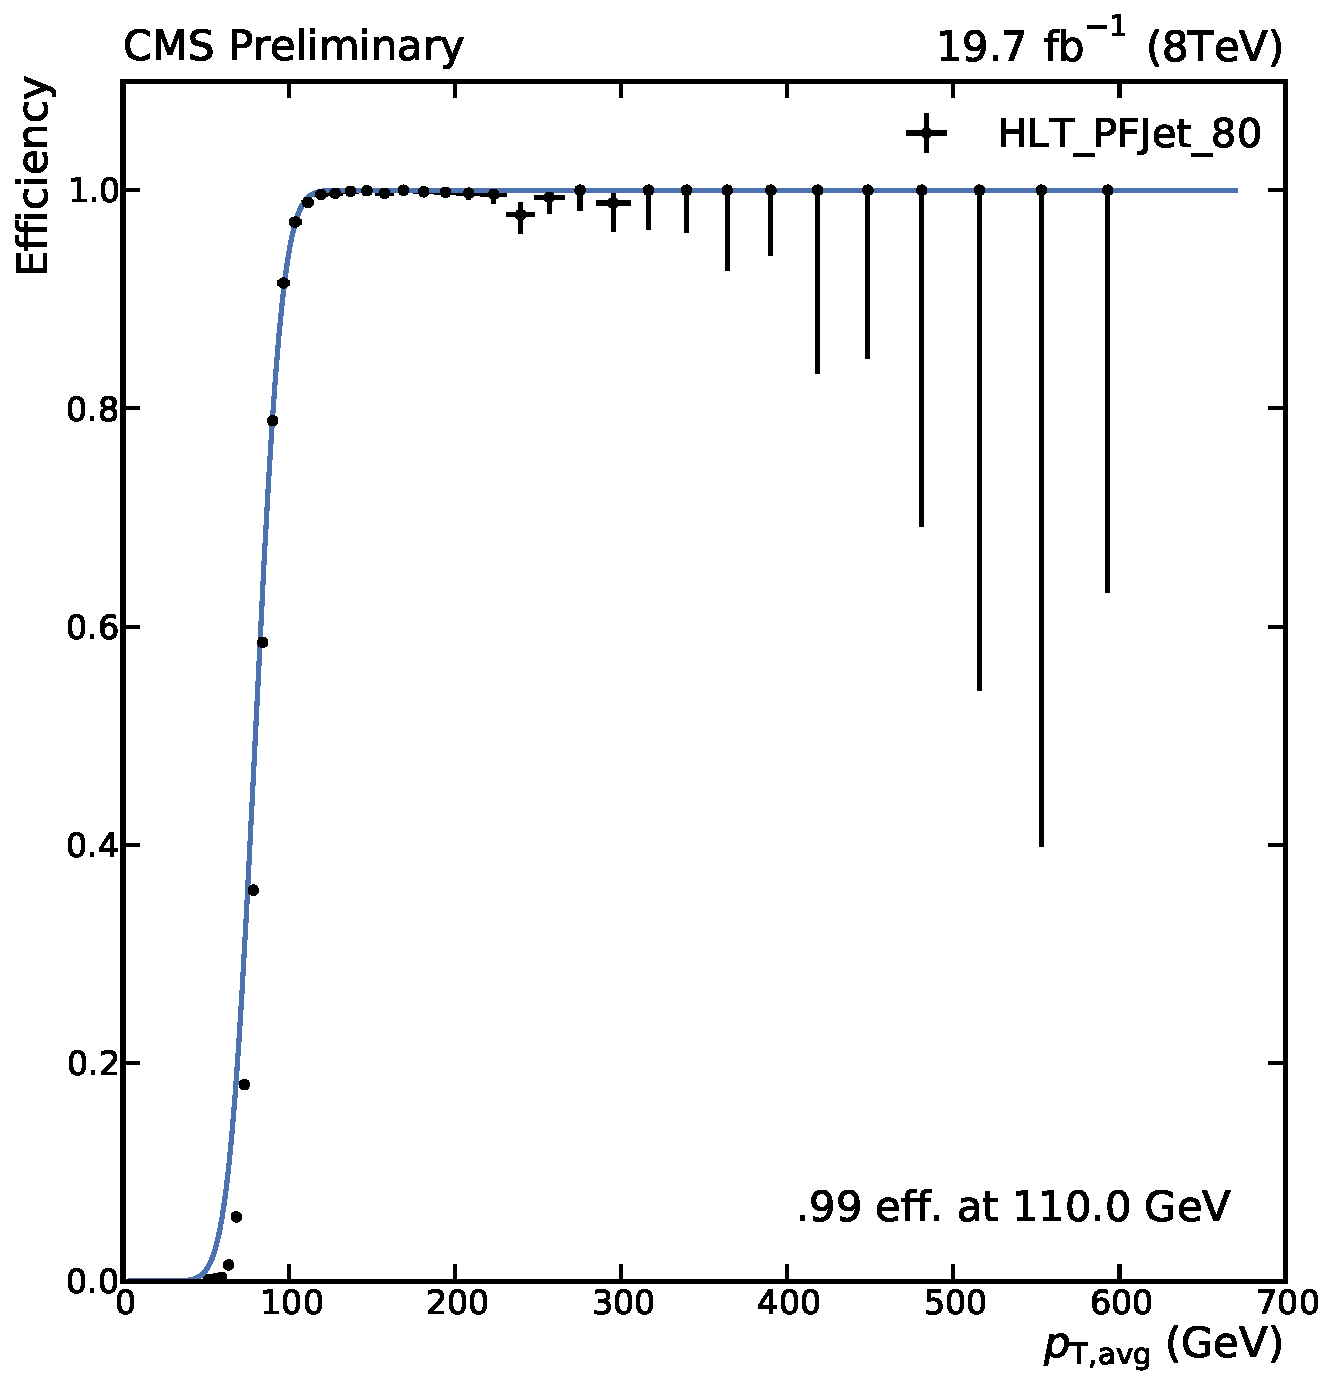
\includegraphics[width=0.45\textwidth]{figures/measurement/trigger_eff_hltpfjet80.pdf}\hfill
    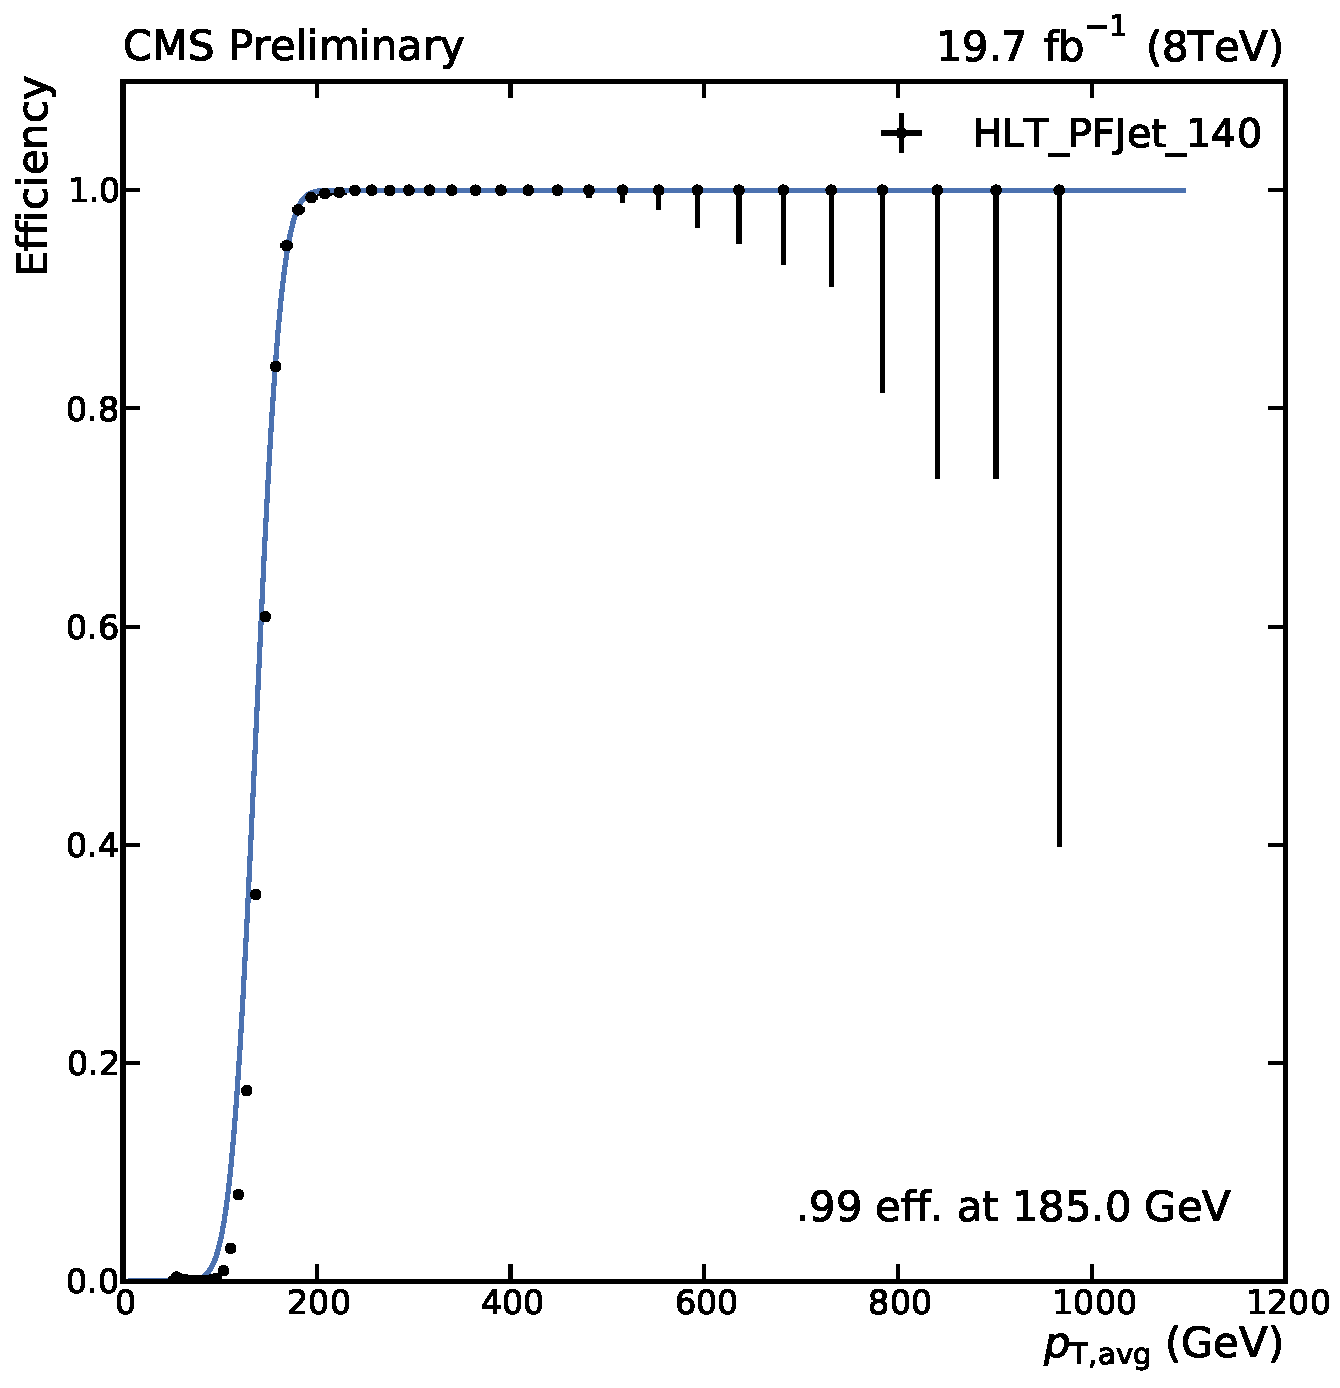
\includegraphics[width=0.45\textwidth]{figures/measurement/trigger_eff_hltpfjet140.pdf}
    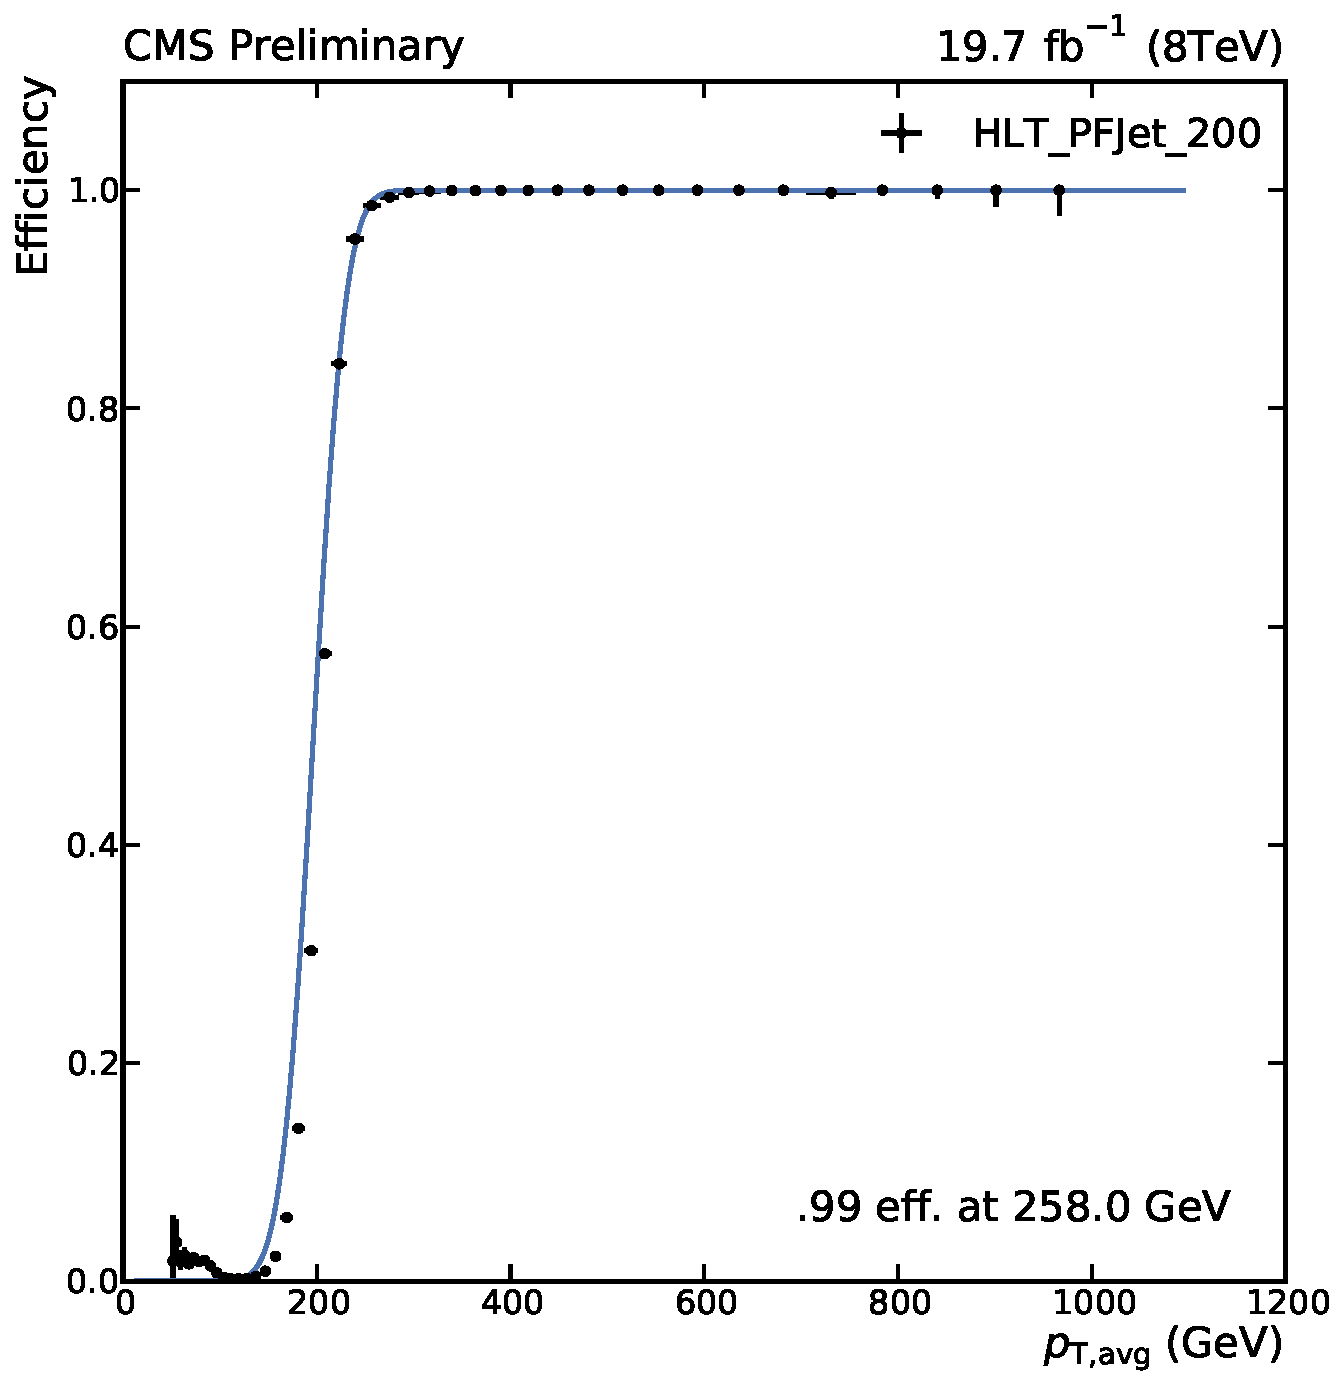
\includegraphics[width=0.45\textwidth]{figures/measurement/trigger_eff_hltpfjet200.pdf}\hfill
    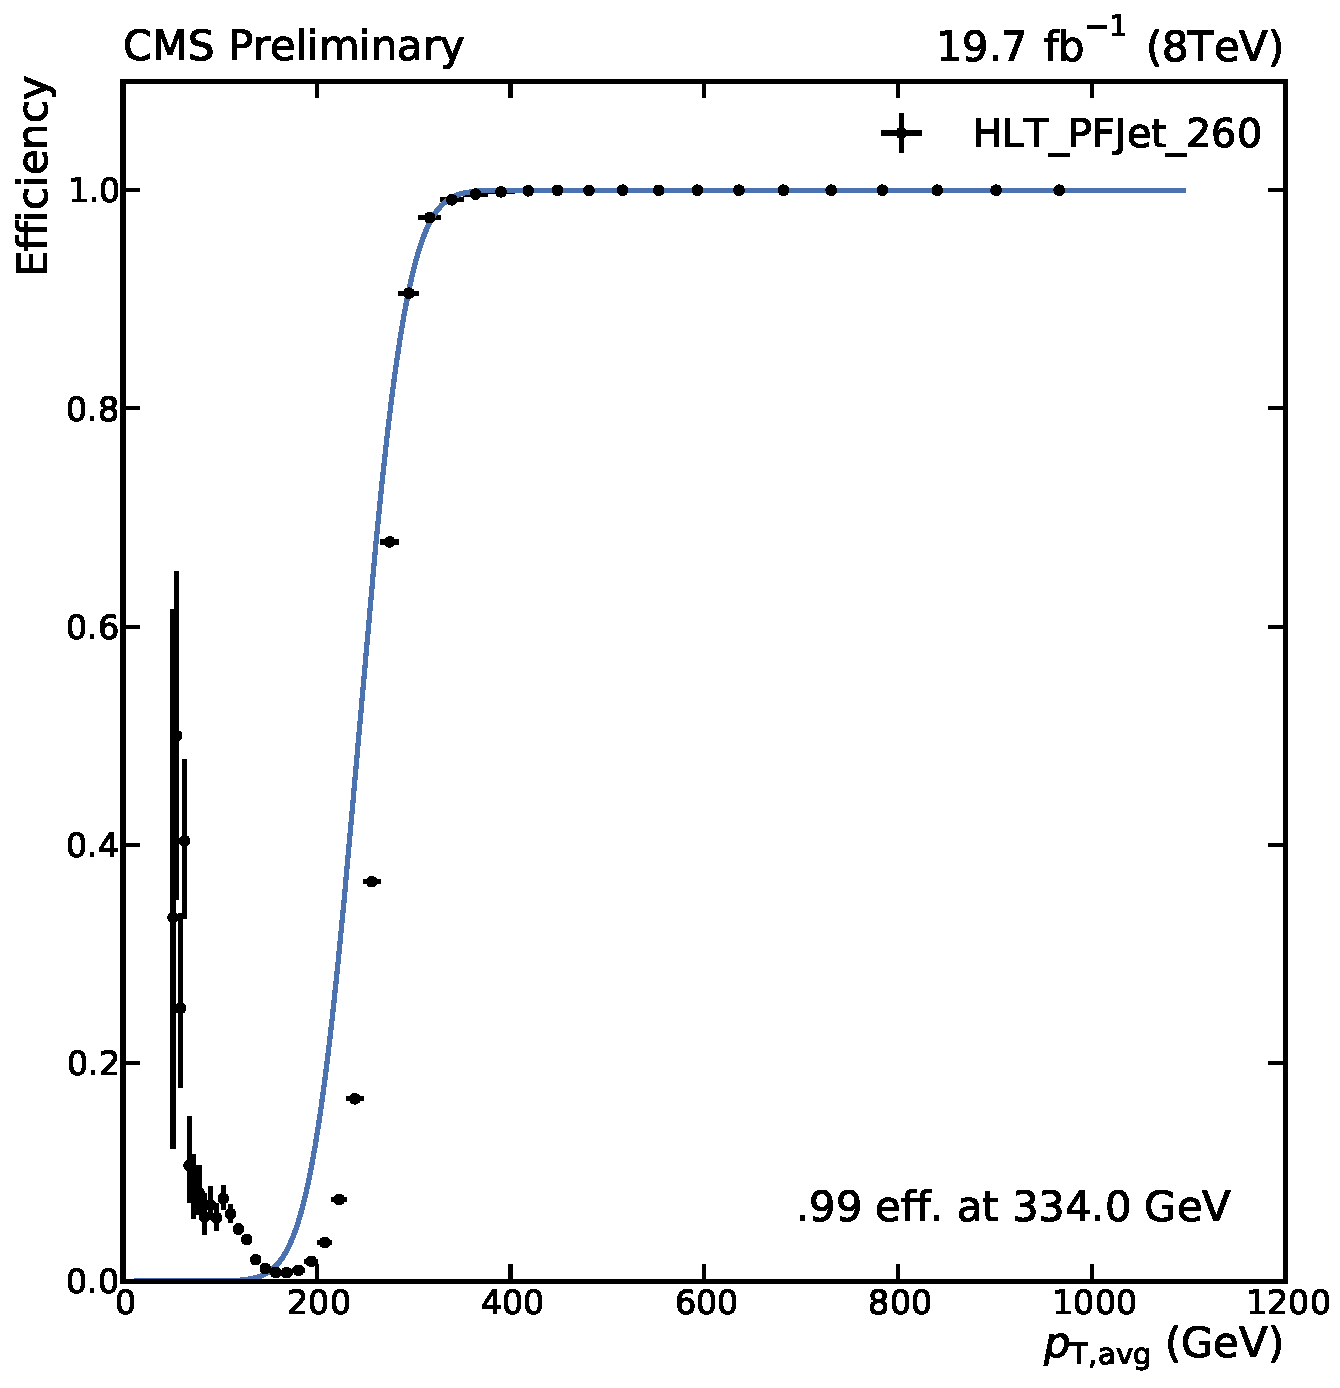
\includegraphics[width=0.45\textwidth]{figures/measurement/trigger_eff_hltpfjet260.pdf}
    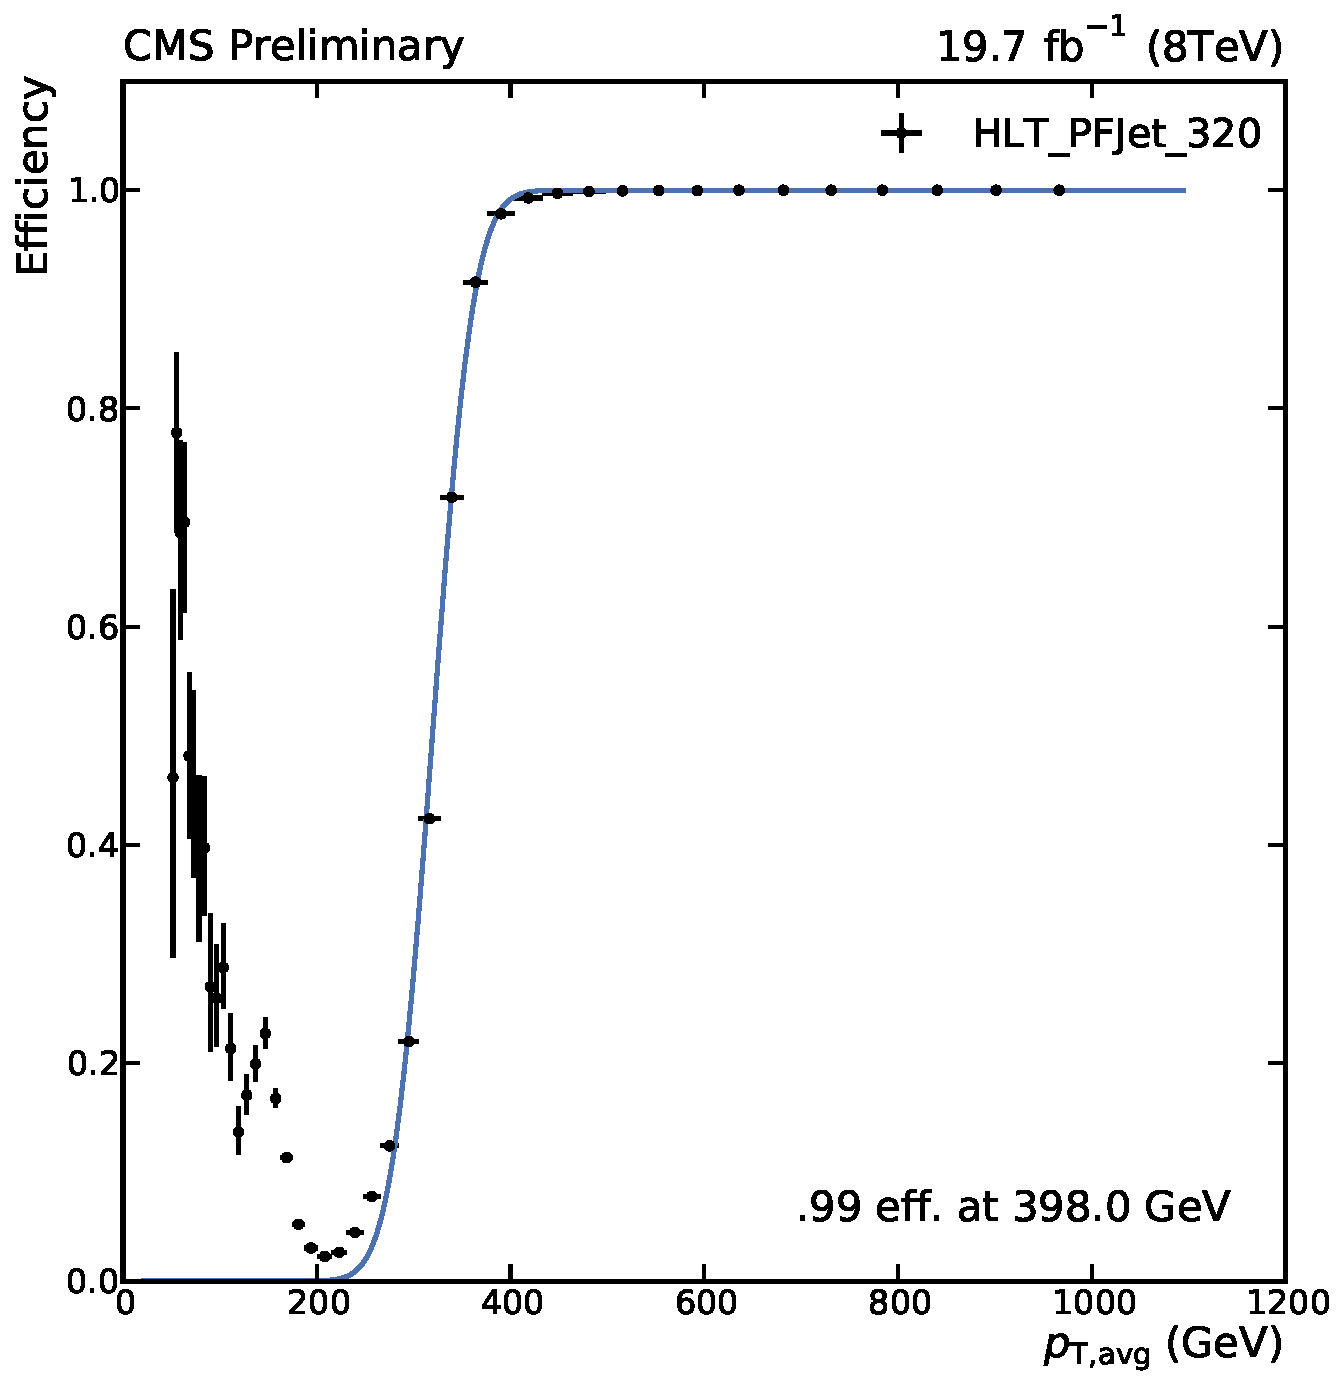
\includegraphics[width=0.45\textwidth]{figures/measurement/trigger_eff_hltpfjet320.pdf}\hfill
    \caption{Trigger efficiencies turn-on curves for the single jet trigger
    paths used in the analysis. To determine the 99\% efficiency threshold, the
    trigger paths are fitted using a sigmoid function taking into account the
    uncertainties using Clopper-Pearson confidence intervals.}
    \label{fig:trigger_eff}
\end{figure}

The reconstruction algorithms and the jet energy corrections applied on HLT
level are slightly different compared to the final data reconstruction.
Additionally the trigger efficiency is not calculated versus $\ptjet$ which was
used in the trigger decision, but versus the \ptavg of the dijet system used in
this analyses. Therefore the trigger paths show a turn-on behaviour as can been seen in
Figure~\ref{fig:trigger_eff} and it is neccessary to determine the threshold at
which a trigger is fully efficient.

Due to the different prescales introduced by each trigger path, it is not
trivially possible to calculate the efficiency by dividing the number of passed events for
one trigger by dividing through the number of events passed by the previous
trigger with the lower \pt threshold which is by definition fully efficient for
the higher trigger path. While it is possible to normalize the yield by the
effective luminosity seen by each trigger, this introduces statistical
fluctuations due to the large differences of the number of events seen by each
trigger caused by the prescale factors.

When the L1 trigger and HLT trigger are processed, the objects passing the
trigger are stored. Therefore it is possible to re-emulate the trigger decision
by comparing the L1 jet \pt with the L1 trigger threshold and the HLT jet \pt
with the HLT threshold~\cite{Stober:2012abc}.

Similarly the trigger decision of the next higher jet trigger can be emulated
starting from the lower trigger path. A set of events $S_1 = \left\{E_i | T_A
(E_i) = true \right\}$ which was accepted  by the lower trigger path $T_A$ is
used to determine the subset $S_2 = \left\{E_i|T_A(E_i) \wedge  T_B(E_i)
\right\}$ which would also pass the higher trigger $T_B$. The ratio of both
event sets can be used to determine the efficiency as shown for each trigger
path in Figure~\ref{fig:trigger_eff} using the Equation~\ref{eq:trigger_eff}.
The error bars of the trigger efficiency are given by Clopper-Pearson confidence
intervals.

\begin{equation}
\label{eq:trigger_eff}
    f_{\text{eff}} (x) = \frac{N(\left\{E_i|T_A(E_i) \wedge T_B(E_i), x)\right\}}{N(\left\{ E_i | T_A(E_i) = \text{true} \right\} , x)}
\end{equation}

The efficiency versus \ptavg is fitted using the sigmoid function~\ref{eq:trigger_eff_fit} describing
the turn-on behaviour of the trigger paths. Each trigger was used in a region in which the efficiency
is larger than $99\%$. The actual used trigger efficiency deviate slightly from the once shown in Table~\ref{tab:triggers}
since the used trigger eff. thresholds were measured for each \ystar and \yboost bin and the most
conservative value was used.

\begin{equation}
\label{eq:trigger_eff_fit}
    f_{\text{fit}} (x) = \frac{1}{2} \left( 1 + \erf \left(\frac{x-\mu}{\sqrt{2}\sigma}\right)\right)
\end{equation}

Table~\ref{tab:triggers} contains the L1 and HLT thresholds of each trigger and
the \ptavg value at which each trigger reaches 99\% efficiency.

\subsection{Primary Vertex Selection}

The \textbf{good primary vertex selection} further rejects beam background and off-centre bunch
crossings. The recommended vertex selection cuts ensure at least one well
reconstructed primary vertex for an event to be further analyzed. The following
criteria are applied 

% Vertex selection
% To reject further beam backgrounds and off-centre parasitic bunch crossings,
% the recommended vertex selection cuts are applied. To pass the step of the
% selection process, an event has to contain at least one well reconstructed
% primary vertex (PV), within a distance of |z(PV)| < 24 cm between the pri-
% mary vertex and the nominal interaction point (IP) of the detector. The
% radial distance ρ(PV) of the vertex from the z axis though the IP is required
% to be smaller than 2 cm, corresponding to the size of the beam pipe. Addi-
% tionally, the fit used to determine the vertex needs to have P
% at least 4 degrees
% of freedom. For an unconstrained vertex fit, which has 2 i w i − 3 degrees
% of freedom (w i ≤ 1), this means at least four tracks with weight ≈ 1 are
% required. The influence of the different steps of the vertex selection is shown
% in table 6.5.

\subsection{Missing transverse energy cuts}

If all particles could be identified and perfectly measured, the sum of the
transverse momenta would sum up to zero. The imbalance in the transverse
momentum of all visible particles, which can be measured in the detector, is
called the missing transverse momentum (MET). Neutrinos, for example, leave the
detector undetected and do contribute to the MET. MET is an important ingredient
in many measurements involving W bosons, top quarks or searches for physics
beyond the standard model which involve undetectable particles. 

A large fraction of the MET is not always caused by physics processes. Very
often the reason can be found in detector noise, cosmic rays or beam-halo
particles. Therefore there are a sequence of algorithms developed by the MET
working group at CMS identifying and rejecting these events. Additionally a cut
was introduced which removes events in which the missing transverse energy
fraction \met constitutes a large fraction of the total transverse energy.

\begin{equation}
    \frac{\met}{\sum_i E_{T,i}} < 0.3
\end{equation}

\subsection{Jet ID selection}

The jet identification criteria rejects noise and noise-enhanced
jets while keeping all real jets. The jet ID is not applied event-wise, but each
jet is accecpted or rejected by the jet id selection. The algorithm works on
particle flow jets using information of the underlying particles. 
Following the recommendations the official loose jet ID is used. Each jet
passing the jet id criteria is then further processed in the analysis chain. The
jet id criteria are based on the properties of each jet. The properties and the
respective cuts are listed in Table~\ref{tab:jetid}. The cut on the neutral
hadron and electromagnetic fractions removes HCAL and ECAL noise. Muons which
are falsely identified and clustered as jets are removed by the muon fraction
criterion. Based on information of the tracker, additional selection cuts are
enforced in the region $|\eta| < 2.4$. Fake jets clustered from electrons are
removed by the charged electromagnetic fraction cut and the charged hadron
fraction must be larger than zero.

While studying the loose and tight jet criteria, it was found that the tight jet
id removes a non-negligible fraction of jets in the forward region of the
phase space considered in this analysis. Therefore the loose jet id was applied.

\begin{table}[htbp]
    \centering
    \begin{tabular}{llll}
    \toprule
                          & Property                & Loose ID & Tight ID\\\cmidrule(lr){2-4}
    Whole $\eta$ region   &                         &          & \\\cmidrule(lr){1-1}
                          & Neutral Hadron Fraction & $< 0.99$ & $< 0.90$\\
                          & Neutral EM Fraction     & $< 0.99$ & $< 0.90$\\
                          & Number of Constituents  & $> 1$    & $> 1$\\
                          & Muon Fraction           & $< 0.8$  & $< 0.80$\\
    Only $|\eta| < 2.4$   &                         &          & \\\cmidrule(lr){1-1}
                          & Charged Hadron Fraction & $> 0$    & $> 0$\\
                          & Charged Multiplicity    & $> 0$    & $> 0$\\
                          & Charged EM Fraction     & $< 0.99$ & $< 0.90$\\
    \bottomrule
    \end{tabular}
    \caption{The jet identification criteria remove fake jets originating from
    detector noise as well as wrongly clustered electrons and muons. Following
    the official recipe, the loose jet id was applied.}
    \label{tab:jetid}
\end{table}

\subsection{Phase space cuts}

\section{Dijet Resolution}

\section{Unfolding}

\section{Uncertainties}
